\documentclass{beamer}

\usepackage{default}
\usepackage[german]{babel}
\usepackage[utf8]{inputenc}                   % replace by the encoding you are using

\usetheme{Berlin}

\newcommand{\cindent}{\hskip20pt}

%Header Settings
%\setbeamertemplate{headline}{}

%Footer Settings
\setbeamertemplate{navigation symbols}{
	\usebeamerfont{footline}%
	\usebeamercolor[fg]{footline}%
	\hspace{1em}%
	\insertframenumber/\inserttotalframenumber
}

\title[Java]{Java - Arrays}
\author[W. Bombardelli]{William Bombardelli}
\institute[Schweizerschule Mexiko]
{
	\vskip 12pt
	Schweizerschule Mexiko, Ciudad de México, Mexico \\
	\texttt{\url{https://github.com/wbombardellis/java-unterricht}}
}
\date{11 March 2020}

\makeatletter
\hypersetup{
	pdftitle = {\@title}, pdfkeywords = {Java}, pdfauthor = {\@author}
} 
\makeatother

\begin{document}
	\begin{frame}
		\titlepage
	\end{frame}
	
	\begin{frame}
		\frametitle{Organization}
		\tableofcontents
	\end{frame}

	%-------------------
	% Arrays
	%-------------------
	\section{Arrays}
	\begin{frame}
		\frametitle{Array}
		Arrays allow you to store several values in one variable
		\pause
		\begin{itemize}
			\item Write a program that reads the grades of ten students and print at the end the average (arithmetic mean) grade and how many students passed ($grade \ge 7$).
		\end{itemize}
		\pause
		$double[]\ grades\ =\ new\ double[10];$\\
		$for\ (int\ i = 0; i < 10; i++)\ \{$\\
			\cindent $grades[i] = reader.nextDouble();$\\
		$\}$\\
	\end{frame}

	\begin{frame}
		\frametitle{Exercises}
		\begin{enumerate}
			\item Now you want your program to send the students' grades to the German Ministry of Education. The problem is that the German grading system is different from the one you use. So extend your program to print the students' grade according to the German system. The grades are translated according to the table below.\\
			\centering
			\begin{tabular}{c | c}
				Mexican 	& German \\
				\hline
				0.0 - 5.9	& 4.0 \\
				6.0 - 6.9	& 3.0 \\
				7.0 - 8.9	& 2.0 \\
				9.0 - 10.0	& 1.0 \\
			\end{tabular}
		\end{enumerate}
	\end{frame}

	\begin{frame}
		\frametitle{Array Grammar Rules}
		\textbf{Array Declaration:}\\
		$\langle Type \rangle []\ \langle Varname \rangle\ =\ new\ \langle Type \rangle [SIZE];$\\
		\vskip20pt
		\textbf{Array Assignment Statement:}\\
		$\langle Varname \rangle [POSITION]\ =\ \langle \text{Expression}\rangle;$\\
		Where $POSITION \in [0, SIZE-1]$.
	\end{frame}

	\begin{frame}
		\frametitle{Exercises}
		\begin{enumerate}
			\item Write a program that reads a word from the keyboard and prints it reversed. Example: Notebook $\to$ koobetoN
			\item Write a program that tells whether a word is a palindrome or not. A palindrome is a word that reads the same backward as forward. Example: level, radar.
		\end{enumerate}
	\end{frame}

	\begin{frame}
		\frametitle{Exercises}
		\begin{enumerate}
			\item Write a program that reads the price of a product and the received money, and prints the amount of change detailed by how many bills of each value to give. Example:\\
			\pause
			\texttt{Price: \$100\\
			Received: \$299\\
			Change: \$199\\
			Change Bills: \\
			1 bills of \$100\\
			1 bills of \$50\\
			2 bills of \$20\\
			0 bills of \$10\\
			1 bills of \$5\\
			2 bills of \$2\\
			0 bills of \$1}
		\end{enumerate}
	\end{frame}

	%-------------------
	% Bidimensional Arrays
	%-------------------
	\section{Bidimensional Arrays}
	\begin{frame}
		\frametitle{Bidimensional Arrays}
		Bidimensional arrays allow you to store a table in one variable.
		\pause
		$int[][]\ table\ =\ new\ int[10][10];$\\
		$table[0][0]\ =\ 23;$\\
		$table[1][2]\ =\ 42;$\\
		\pause
		$for\ (int\ i = 0; i < 10; i++)\ \{$\\
			\cindent $for\ (int\ j = 0; j < 10; j++)\ \{$\\
				\cindent \cindent $System.out.println(table[i][j]);$\\
			\cindent $\}$\\
		$\}$\\
	\end{frame}

	\begin{frame}
		\frametitle{Image Processing - Filters}
		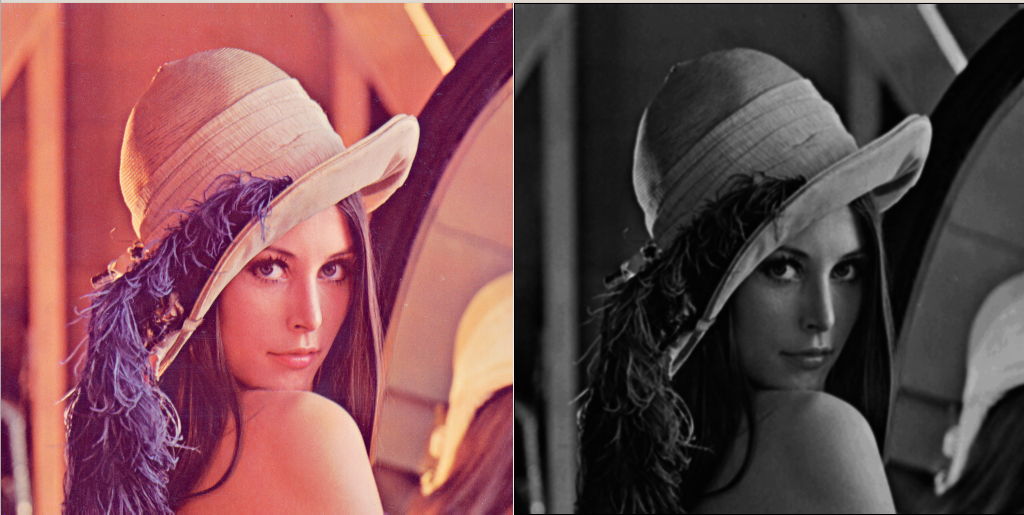
\includegraphics[width=\textwidth]{lenna.png}
	\end{frame}

	%-------------------
	% Summary
	%-------------------
	\section{Summary}
	
	\begin{frame}
		\frametitle{Summary}
		\begin{itemize}
			\item Arrays allow you to store several values in one single variable.
			\item Next Lesson: Assignment
		\end{itemize}
	\end{frame}

	\begin{frame}
		\frametitle{References}
		\begin{itemize}
			\item W3C Tutorial: 
			\begin{itemize}
				\item \url{https://www.w3schools.com/java/java_arrays.asp}
			\end{itemize}
			\item Exercises: \url{https://www.w3schools.com/java/exercise.asp}
			\begin{itemize}
				\item Java Arrays
			\end{itemize}
		\end{itemize}
		
	\end{frame}

\end{document}
